\section{Software Implementation}
In this section, the actual implementation of the software has been detailed, including: what tools were used in the implementation, how the software was implemented, and any issues that were encountered during the implementation process.
%{\color{red}

%\begin{enumerate}
%\item simple introduction to the program, what it does and who it is for
%\item technical solution adopted, what technical solution has been implemented, whether it is ideal, whether an alternative exists
%\item software engineering information, program design, structure, definition language, test plans
%\item development approach used (evolutionary, build and fix)
%\item Problems encountered (bugs, errors, uncompleted sections of code)
%\item hardware/ software requirements
%\item Friendly errors
%\item Help system is dedicated, but offers links to other, helpful, external resources
%\end{enumerate}

%}

\subsection{Key Implementation Decisions}
\label{sec:kid}
As detailed in section \ref{sec:pat}, there were many different potential platforms and tools can could have been used in the implementation of the project. In this section, the final decision for which tool to use for each distinct section of the project has been detailed, along with their justifications.

\tocless\subsubsection{System Back End - R-Shiny}
R-Shiny is a new, up and coming R Package, that allows for the creation of web applications using the R programming language. The main reason that R-Shiny was selected as the back end was that it would be able to use the FuzzyToolkitUoN R package, and access all the fuzzy logic inferencing tools that were contained within it. R-Shiny was chosen over R-Node due to, at the time of implementation, R-Node not having a working website, and thus no ability to actually download it; which is not the sign of a well-maintained tool. Node.js was not chosen as this would require a brand new inference engine to be written in JavaScript, which would have taken a considerable length of time, and may not have been completed during the life time of the project.\ \\
\ \\
Unfortunately, as detailed in section \ref{sec:pe}, this may have not been the greatest choice, as some issues were discovered with R-Shiny. However, the ability to use the FuzzyToolkitUoN inference system was a vital part of the project, and as R-Shiny continues to be developed, hopefully these issues will be resolved.

\tocless\subsubsection{Front End Programming Language - JavaScript}
JavaScript is a client-sided programming language used to dynamically alter the content of an HTML document. This the perfect tool to be used, as it has the ability to directly and easily manipulate the content of a web page, and thus dynamic interfaces can be constructed with ease. It also fulfils the goal of the system being easy to access, and use, as the user is not required to install any extra software, to begin using the system (like they would have to have done, if the other alternative, Adobe Flash, was used instead). Using JavaScript also means that other JavaScript libraries could be used within the system, and thus greater functionality provided. One other JavaScript library heavily used within the system is JQuery, which is a fast, small, and feature rich JavaScript library, that greatly simplifies document traversal and manipulation, and event handling.

\tocless\subsubsection{Front End Design Framework - Twitter's Bootstrap}
Despite complaints that Bootstrap is overused, it is still by far the best front end design framework available. This is due to ease of use, huge number of UI elements to choose from, and extensive documentation. Many of Bootstrap's feature were included in the implementation of the project, to heighten the user experience. This included the use of modal windows to reduce on-screen clutter, coloured buttons to dictate functionality, and tabbed panes, to help split the system into smaller segments. Due to the adoption of Bootstrap, the system is also fully responsive. This means that the system automatically scales to work on any screen resolution, from large, to small. This makes the system much more accessible to all users, and no strange UI bugs will occur if the user is using a different screen resolution to the one the system was designed on. \ \\
\ \\
The only negative of using Bootstrap is that the modal window class does not function correctly when viewed on a mobile device. However, this is not a huge issue, as the system isn't truly designed to work on mobile devices, as this is an impractical interface for designing a fuzzy system. 

\tocless\subsubsection{Graphing Tools - Google Charts/Directly from R}
Of the three potential candidates for graphic tools, Flot, was ruled out, due to it being difficult to use, and having a limited number of graph types available. The system instead utilised Google Charts for the majority of chart drawing. This is because Google Charts provide aesthetically pleasing, interactive graphs, in a large number of formats, and has extensive documentation. The graphs drawn to represent the fuzzy sets in the membership function creator, and those in the variable creator are all drawn using Google Charts.\ \\
\ \\
Unfortunately, Google Charts does not support the drawing of three dimensional graphs, whereas FuzzyToolkitUoN does. When a fuzzy system of two inputs, and one output is defined (a common set up for type-1 systems), a three dimensional surface plot of the mapping between the two is an extremely effective way of visualising the system. For this reason, on the evaluation page, if the user has specified a system of two inputs and a single output, a surface plot will be displayed, directly from R.

\subsection{Implementation Methodology}
% agile - scrum - kanban ( but with trello ) 
To help manage the implementation of such a large piece of software, the adoption of some methodology was necessary. It was decided that the best methodology would be an agile one, with heavy use of Kanban, using the tips laid out by Henrik Kniberg \cite{kniberg2007scrum}. In order to accomplish this, at the beginning of the implementation stage, after the requirements specification had been detailed, the entire project was split into user stories. Each of these stories detailed a specific action that a user of the system would be able to accomplish, along with how long it should take to implement, how important it was, and a way of testing its completion. These stories were then organised onto a digital Kanban Board, using a service called Trello\footnote{\url{http://www.trello.com}}. \ \\
\ \\
Each week, a set of tasks would be selected to be worked on for that week. The amount of tasks selected would be dependent on how much was completed, on average, in the weeks before, so that reasonable estimates could be made (obviously excluding the first few weeks). This ensured a decent portion of work was being completed per week, and that progress was constant. During the week, tasks would be selected from the available pool, prioritising those that were prerequisites of others, or had a high importance, and would then be worked on until completion. After the completion of a task, a new task would be selected, and work would begin on this. This was an extremely effective method of managing the implementation, as any small tasks that were necessary could be added to the board, and there was an assurance they would eventually be completed, and nothing would be overlooked.

\newpage 
\subsection{Detailed Description of the User Interface}
In this section, each individual screen of the system has been displayed, along with a detailed explanation of why it is effective, and why it has been implemented as it has.\ \\
\ \\
The first screen presented to the user upon launching the system (shown in figure \ref{fig:ss-ui-0}), is a greyed out version of the input creation page, with a modal window displayed. This modal window gives a brief explanation of the purpose of the system, how to get started, the intended audience, and contact details for the maintainer. The purpose of this is so that any user that has navigated to the website can very quickly gain an understanding of what the system is for, how to use it, and as a result, whether or not they would want to, or need to.

% What screen it is
% Explain individual elements about it. Why are they good?
% Why was it implemented in this way?

\begin{figure}[ht!]
	\centering
	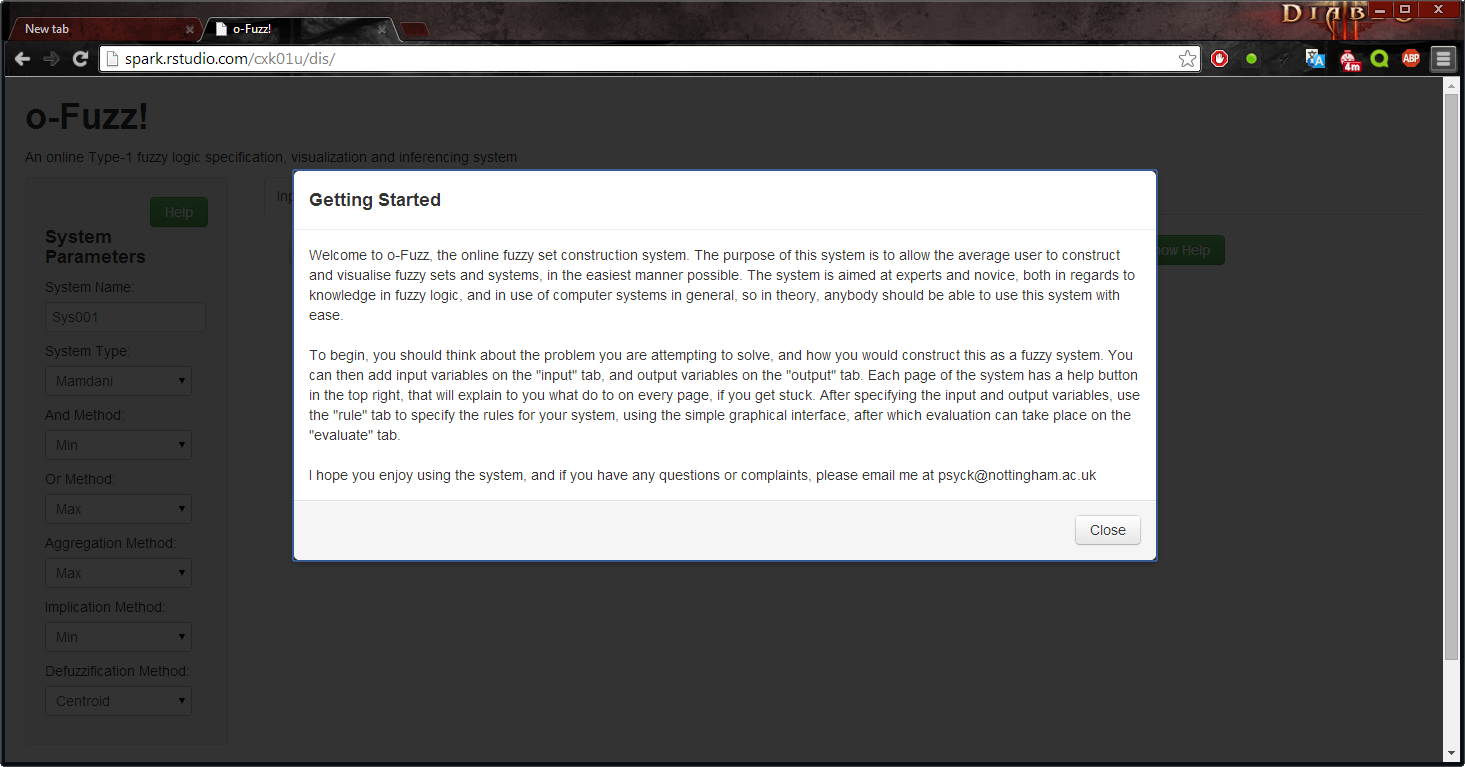
\includegraphics[width=0.75\textwidth]{images/ui-0}
	\vspace{-2mm}
	\caption{Screen shot of initial landing page modal window}
	\label{fig:ss-ui-0}
	\vspace{-1mm}
\end{figure}
\noindent 
After the user has finished reading the initial modal and closed it, they will be presented with the input variable creation screen. Inputs are generally the first thing a user will create in their system (as this is logically first), so this is a perfect landing page. The system wide parameters are also displayed on the left hand side of this page, which is where the eye of the user will be drawn to first, and thus noticed. A screen shot of this page, with two collapsed input variables, can be seen in figure \ref{fig:ss-ui-1}. As you can see, all of the buttons on the page stand out, and can be easily located. This means the user's attention can cycle between the buttons easily, greatly increasing the speed at which they can accomplish their tasks. The help buttons, in green, are consistently displayed in the top right hand corner of the section they are providing help for, making them extremely easy to find, if help is required.

\begin{figure}[ht!]
	\begin{center}
		\fbox{
		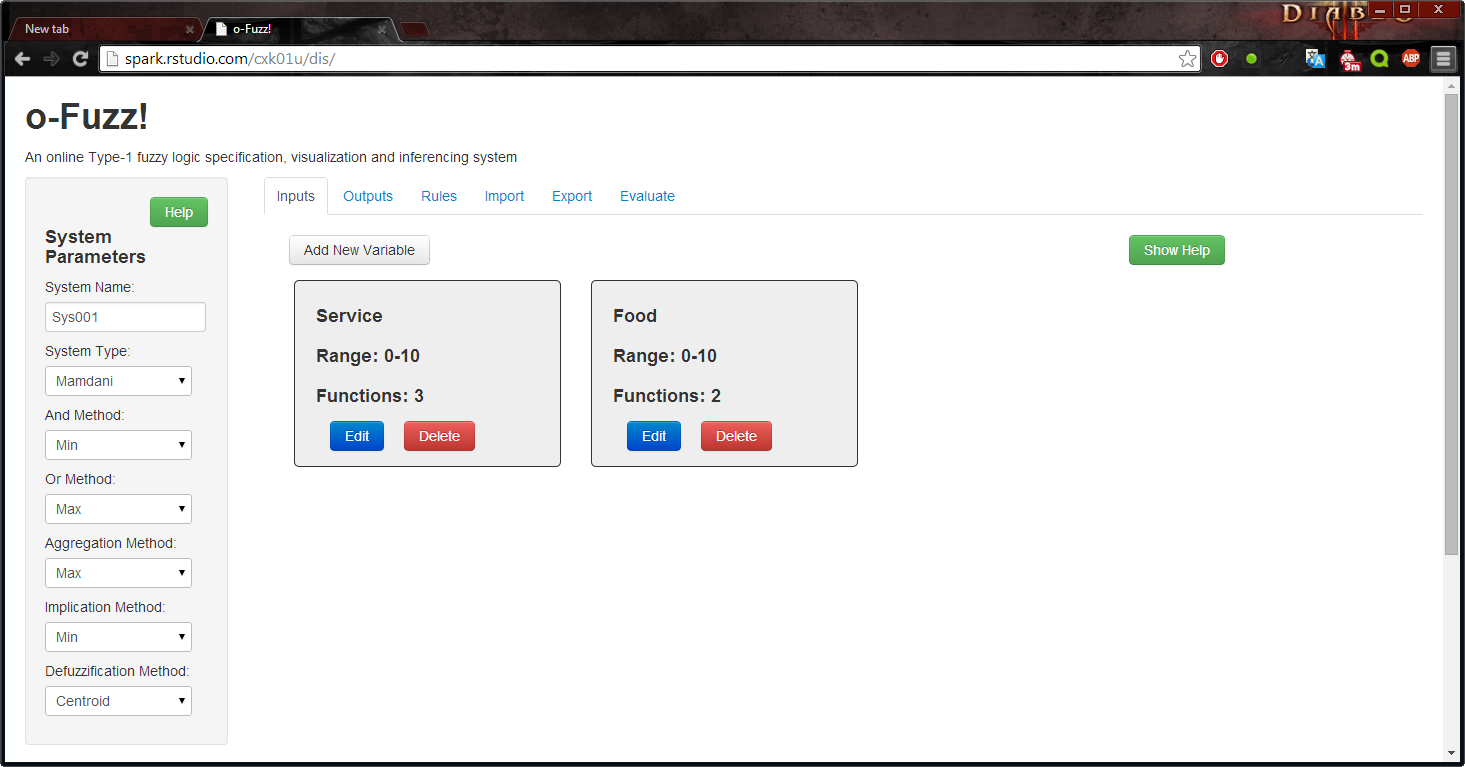
\includegraphics[width=0.85\textwidth]{images/ui-1}
		}
	\end{center}
	\vspace{-6mm}
	\caption{Screen shot of the input variable creation screen, with collapsed variables}
	\label{fig:ss-ui-1}
	\vspace{-10mm}
\end{figure}
\noindent
Upon clicking the ``Edit'' button of a collapsed variable, the expanded view of it would be displayed, as shown in figure \ref{fig:ss-ui-2}. In this expanded view, all the information of the variable would be displayed, such as the name, range, and any membership functions. These properties were now also editable, which they were not in the collapsed view. This means that to make a change, the user has to actively click a button, which decreases the chance of this happening by mistake. In this expanded view, the same colour scheme is observed as with the rest of the web site: blue representing editing or modifying, green representing a positive action, and red representing a negative action, like deleting. A plot of the membership functions of the variable can also be seen in the expanded view, which allows the user to visualise this variable, and all of the membership functions it contains alongside one another.
\begin{figure}[ht!]
	\begin{center}
	\fbox{
		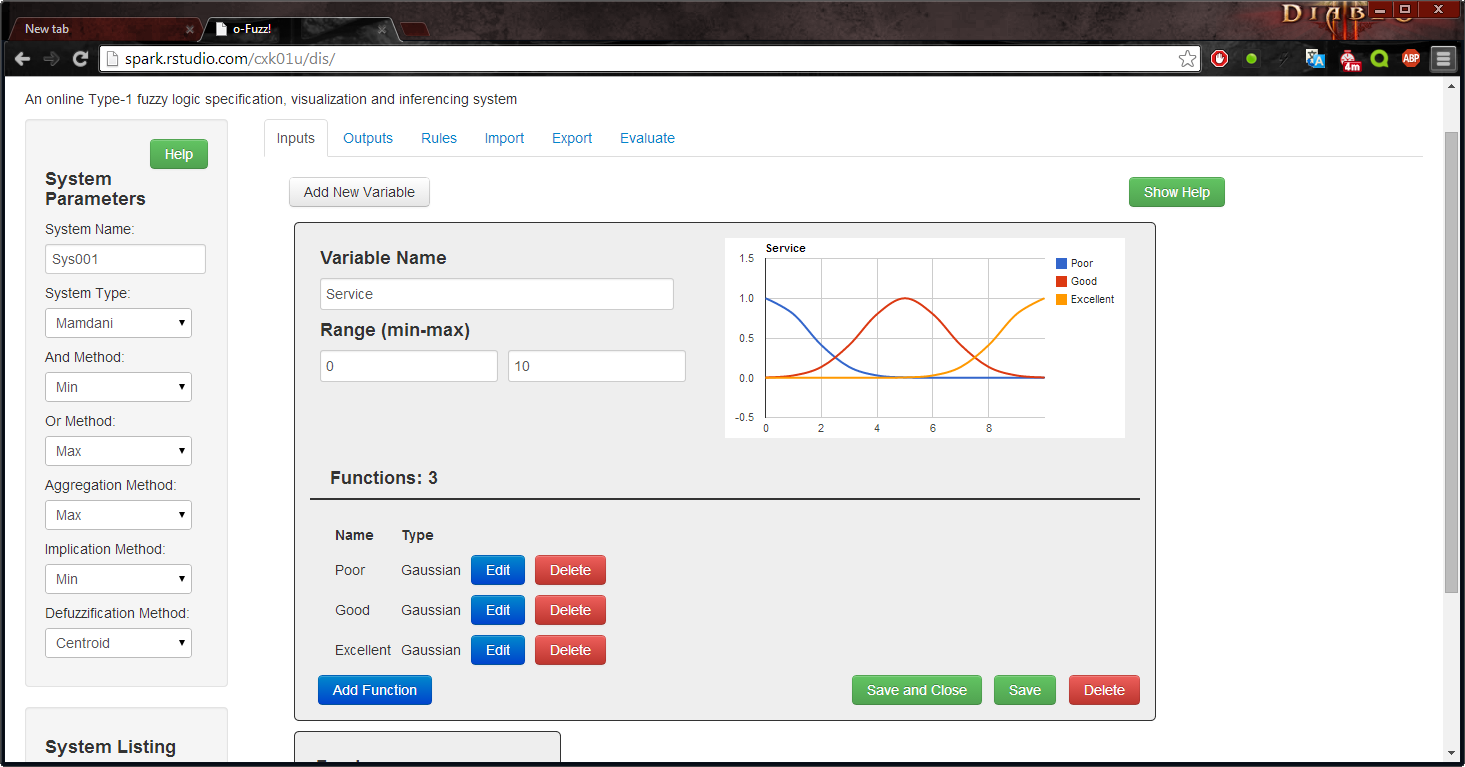
\includegraphics[width=0.85\textwidth]{images/ui-2}
	}
	\end{center}
	\vspace{-6mm}
	\caption{Screen shot of the input variable creation screen, with expanded variable}
	\label{fig:ss-ui-2}
\end{figure}

\noindent 
Upon clicking the ``Add Function'', or ``Edit'' buttons on the expanded view, the membership function creation window would be displayed (seen in figure \ref{fig:ss-ui-4}).


\begin{figure}[ht!]
	\begin{center}
		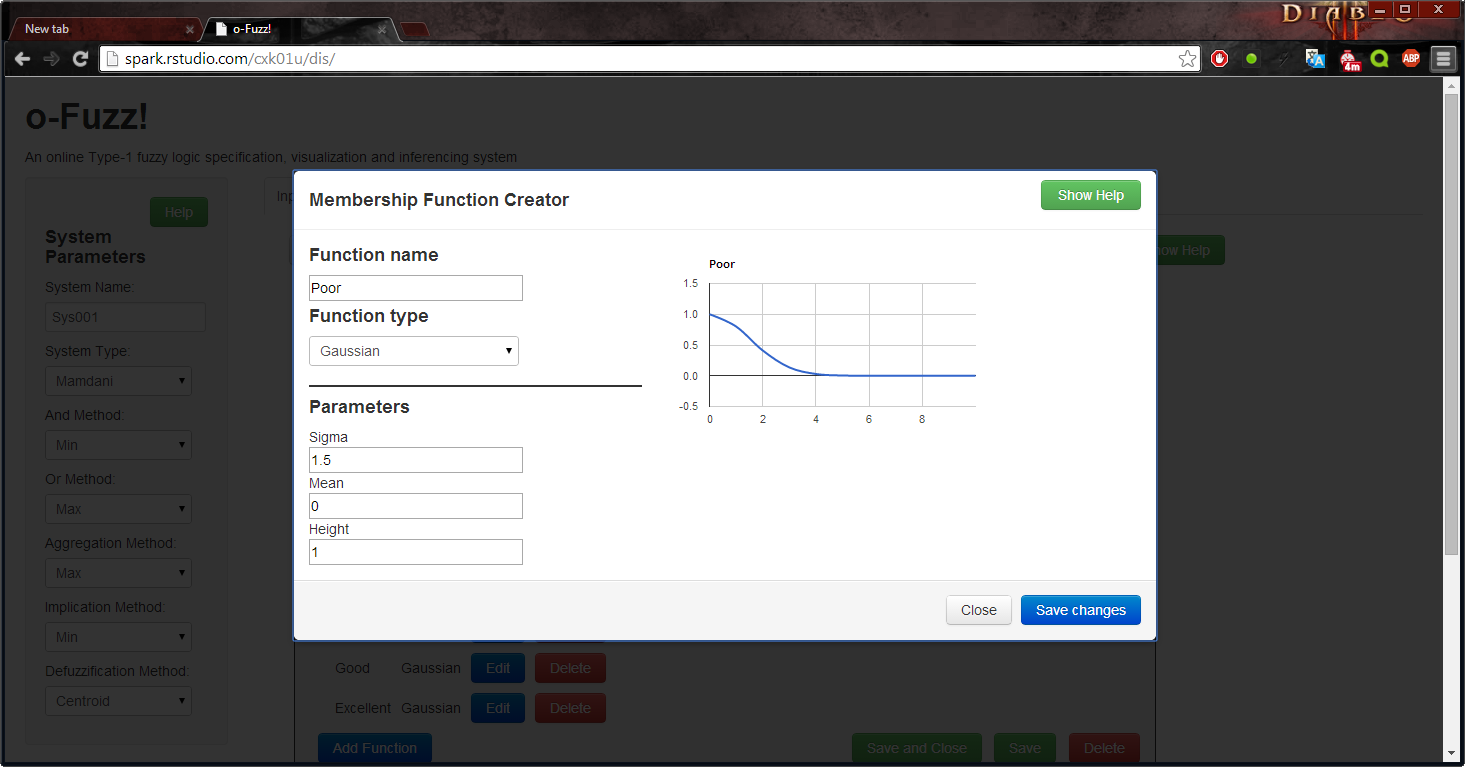
\includegraphics[width=0.75\textwidth]{images/ui-4}
	\end{center}
	\vspace{-6mm}	
	\caption{Screen shot of the membership function creation modal}
	\label{fig:ss-ui-4}
	\vspace{-6mm}	
\end{figure}

\noindent
The reasons for this being in a separate window are that it helps to split conceptually distinct tasks, reduces cognitive load on the user, and decrease clutter on the user interface. On this screen, the user is able to specify the parameters for a fuzzy set, and see how this set looks, once all parameters have been specified. This graphical representation is extremely useful for the user, as they can inspect their creation, and ensure it is as they expected. Note that the help button remains consistently placed in the top right hand corner.\ \\
\ \\
After creating the input variables, and the output variables (whose interface is exactly that of the input variable, and thus has not been shown), the user would logically move onto the creation of rules. The interface for this, is displayed in figure \ref{fig:ss-ui-5}. On this page, you can see that the consistent colour scheme has been kept, with the edit buttons being blue, the delete buttons being red, and the help button being green, and in the top right hand corner. On this screen, the rules that have been created will be displayed, in plain English, to the user, with the ability to edit and delete them. This is a much more intuitive way to display the rules than, for instance, FuzzyToolkkitUoN, which simply represents rules as a list of numbers. As this system is comprised of two inputs and one output, rule tables are also drawn for the user, to help them visualise all of their rules at once.

\begin{figure}[ht!]
	\vspace{-2mm}
	\begin{center}
	\fbox{
		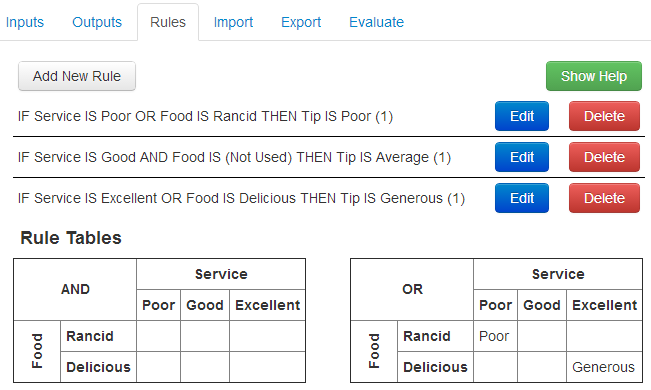
\includegraphics[width=0.625\textwidth]{images/ui-5}
	}
	\end{center}
	\vspace{-6mm}
	\caption{Screen shot of the rule management page}
	\label{fig:ss-ui-5}
	\vspace{-2mm}
\end{figure}

\noindent
Like the creation of membership functions, the creation of rules takes place in a separate window (shown in figure \ref{fig:ss-ui-6}). This is to help the user understand that these are distinct operations, reduce cognitive load, and reduce clutter on the interface. The window itself helps to make the task of creating rules as simple as possible, by only requiring the user to select a term for each variable, from a drop down box. The rule itself is also displayed at all times, so that the user knows exactly what they are creating.

\begin{figure}[ht!]
	\begin{center}
	\fbox{
		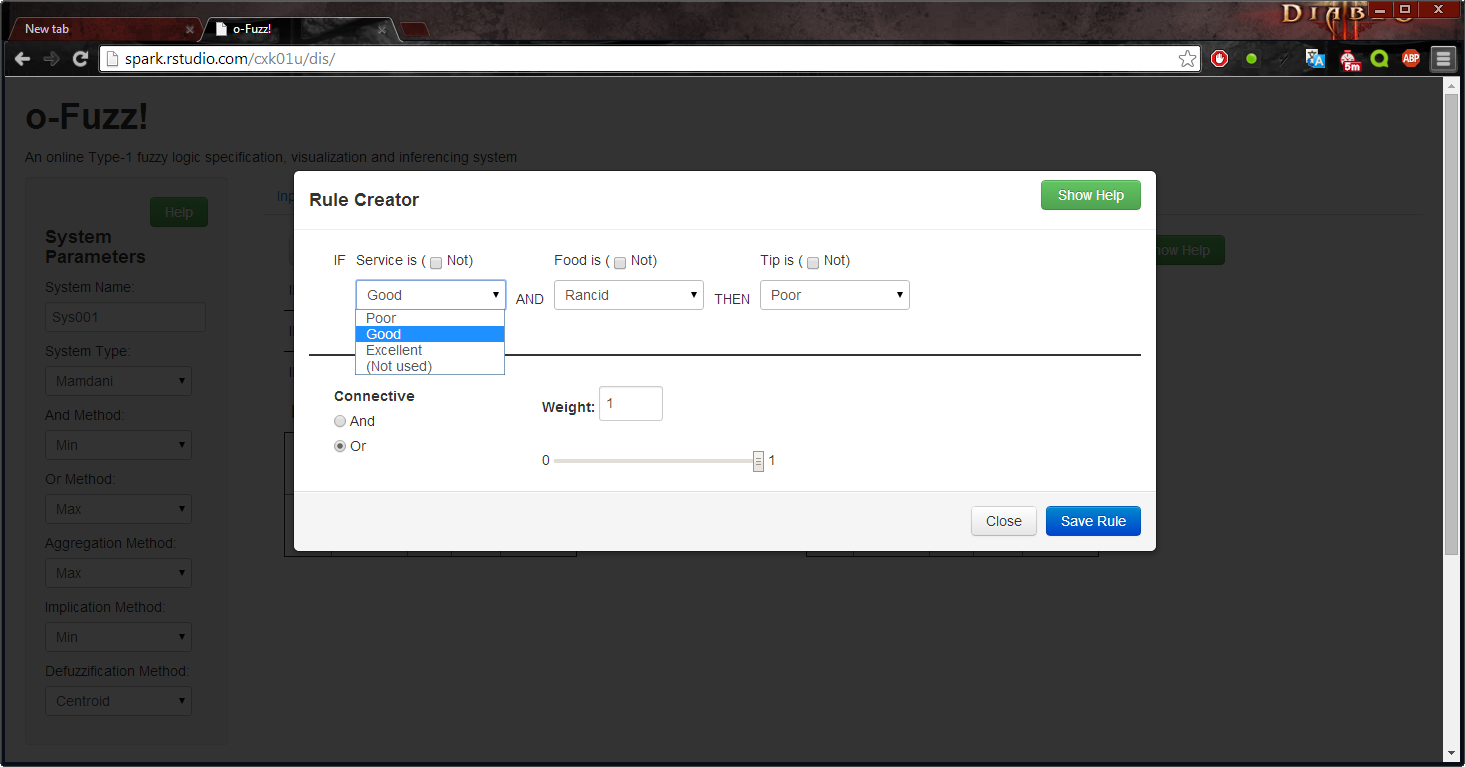
\includegraphics[width=0.6125\textwidth]{images/ui-6}
	}
	\end{center}
	\vspace{-6mm}
	\caption{Screen shot of the rule creation modal}
	\label{fig:ss-ui-6}
	\vspace{-7mm}
\end{figure}


\noindent
After the inputs, outputs, and rules have been specified, the user is finally ready to evaluate their system. This screen can be seen in figure \ref{fig:ss-ui-9}. Each of the inputs, and their potential range, can be seen on the left, with the corresponding output on the right. In addition to this, because the system has two inputs and a single output, a three dimensional surface plot of the system (that is generated directly in R) is also displayed, so the user can easily visualise the mapping between all pairs of inputs, and their output.
\begin{figure}[ht!]
	\begin{center}
	\fbox{
		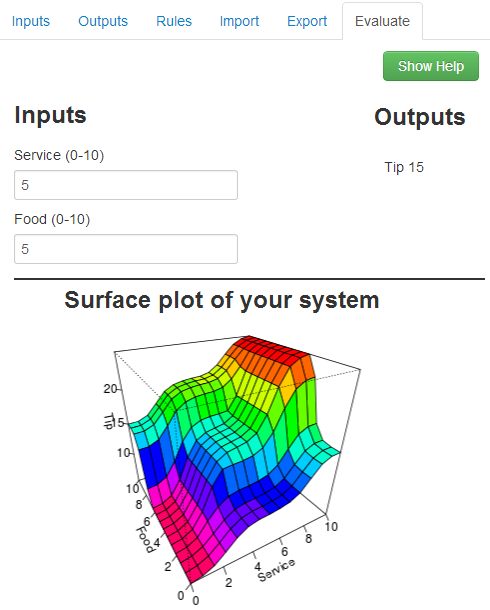
\includegraphics[width=0.5\textwidth]{images/ui-9}
	}
	\end{center}
	\vspace{-6mm}
	\caption{Screen shot of evaluation page, with surface plot}
	\label{fig:ss-ui-9}
	\vspace{-3mm}
\end{figure}


\noindent
After evaluating their system, the user may wish to import another file to evaluate, or even save their current file, both of which they are able to do (in fact, they can do this at any point, due to the flexible navigation system). The interface for importing files is displayed in figure \ref{fig:ss-ui-7}. This is the simplest of all pages of the website, and has a single button present. This makes the task of importing files very simple, because there are no other buttons to press. Once pressed, a file dialogue is launched, and the user can select a MATLAB FIS file, a FuzzyToolkitUoN FIS file, or an o-Fuzz JSON file to be imported. This is then loaded into the system, and also display on this screen, so the user can be assured this is the file they wanted, and that it loaded correctly.

\begin{figure}[ht!]
	\begin{center}
		\fbox{
			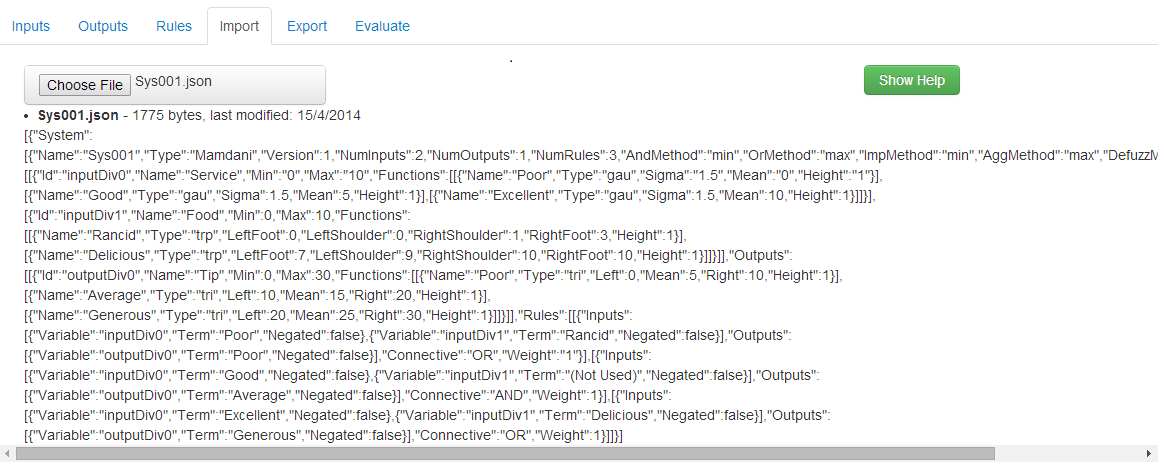
\includegraphics[width=0.9\textwidth]{images/ui-7}
		}
	\end{center}
	\vspace{-6mm}
	\caption{Screen shot of file import screen, with JSON file loaded}
	\label{fig:ss-ui-7}
	\vspace{-3mm}	
\end{figure}

\noindent
The final screen of the system is the file export page. Like the file import screen, this is an extremely simple page, making it very easy to use. This page has two buttons, one that generates a file to be exported (from three options), and another to actually download this file. Initially, the download button is disabled, until the user has selected a file type. After which, it will turn blue (indicating it is now usable), and the user will be able to download their file. This can be seen in figure \ref{fig:ss-ui-8}.

\begin{figure}[ht!]
	\vspace{-1mm}
	\begin{center}
		\fbox{
			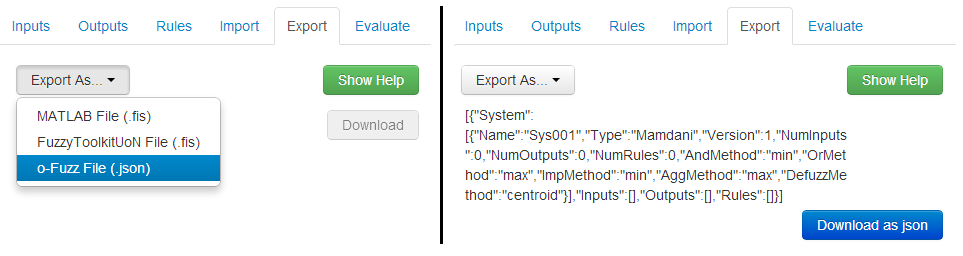
\includegraphics[width=0.99\textwidth]{images/ui-8}
		}
	\end{center}
	\vspace{-6mm}
	\caption{Screen shots of file export screen, before and after selecting a file type}
	\label{fig:ss-ui-8}
\end{figure}




\subsection{Implementation of System Components}
\tocless\subsubsection{Web Front End}
The front end of the project was written in HTML 5, with CSS 3 for styling (most of which was obtained from BootStrap). The dynamic interface and functionality of the system, were provided by a mixture of JavaScript, and JQuery. The purpose of the front end was to provide the user access to powerful back end inferencing tools, via an extremely simple user interface, to facilitate both novice and expert users. There were some 4,100 lines of JavaScript/JQuery across 10 individual files in the final copy of the software. Each file dealt with a very specific part of the system, as to help split up the huge code base into manageable chunks (for instance, one file would deal entirely with rules, whereas another would deal with file importing and exporting).\ \\
\ \\
The front end is certainly a strong point with the system, as it has a clean, uncluttered interface, but also provided a wide range of functionality. Due to the modularity of code, adding new functionality is also extremely easy, and the consistent commenting through the files makes finding key functions (whether this be for debugging, or when extending the system) very easy, and understanding them equally so. Of course, with any interface, there is potential for improvement, to better suit users. For instance, the system could have had customisation possible, to help make the system appeal to different sets of users, or it could have had more support for keyboard short cuts. More detail on this can be found in section \ref{sec:mui}.

\tocless\subsubsection{R-Shiny Back End}
The back end of the system was constructed using R-Shiny, interacting with the FuzzyToolkitUoN R package, and thus was written entirely in R. This gave the system access to the powerful processing tools that R provides, and the visualisations that it can provide, if necessary. The purpose of the R-Shiny segment was to gather the data the user input into the front end, turn this into a format that could be used by the FuzzyToolkitUoN package, and then call the necessary functions for processing to take place.

\newpage 
\noindent 
The biggest issue with using R-Shiny is that it was a tool still in development, and there were some bugs present, and features missing. The biggest of these was the inability to properly handle dynamic user interfaces, such as the one this system required. This meant that, when it came to handling the user input, a hack had to be put in place for this to be dealt with correctly. This is covered in greater detail in section \ref{sec:pe}.

\tocless\subsubsection{Front and Back End Interaction}
\noindent 
The interaction between the front and back ends is extremely important for this system, as it meant that the user input could be dealt with on one side, and the processing of this input on another. The front end allowed for the user to fully specify their fuzzy system, including inputs, outputs, rules, and system parameters, and the back end would take these values, and evaluate the system, and return the appropriate results.\ \\
\ \\
When the user navigated to the export tab, or the evaluate tab, the front end would query the arrays that were holding the system inputs, system outputs, and system rules, and combine these into a string, of the same format as a FuzzyToolkitUoN FIS file. This would then be stored in a text box, hidden from the view of the user. The back end of the system could then index into this hidden text box, and extract the value from it. After some parsing, this object would be converted into a FIS object that the FuzzyToolkitUoN package could handle, and then evaluation, or file exporting, could occur.

\subsection{Problems Encountered}
\label{sec:pe}
Unfortunately, as with most software systems, the implementation stage of this project was not without it's problems; the first of these being with the back end tool that was chosen, R-Shiny. As R-Shiny is a relatively new R Package, support for it is limited. This means that any issues that arise whilst attempting to use it, may not be documented, and a solution not found. The main issue that arose in this particular project, was the difficulty of creating a dynamic user interface, that may interact with R-Shiny. Normally, R-Shiny expects a static user interface, which allow for the server to index specific UI elements, and return their value. Unfortunately, that would not work for this project, as lots of dynamic UI elements were necessary, so that the user could construct the system exactly as they required. This meant it was impossible to list all UI elements in the server, as there could be any number. This problem was not discovered until a great deal of work had been carried out on the front end side, and at a point in the project life time at which restructuring was simply not possible. \ \\
\ \\
A solution to this problem was eventually arrived at, although it was not ideal. Instead of attempting to return the value of every single UI element that could possibly be created in the system, a hidden call-back UI element was included. This call-back UI element was hidden from the user, but would be populated, using JavaScript to loop through all UI elements, with details of the system the user had created whenever server side interaction was required. This meant that the server was required to parse the input it received, but this was a trivial task.\ \\
\ \\
Another issue that arose multiple times throughout the project, was the difficulty of working with such a large code base. By the end of the project, there was approximately 4,000 lines of code (split between R, and JavaScript), across 10 individual files. This could make debugging sometimes extremely difficult, as there was often a chain of function calls that would pass through multiple files, making pin-pointing exactly where errors occurred very troublesome.\ \\
\ \\
Luckily, the Google Chrome JavaScript debugging functionality is very powerful, and would highlight the file that the error originated in. This meant that tracing the calls backward was much simpler, and errors be fixed much quicker. Google Chrome also allowed for the inspecting of variables being passed throughout the system, which meant values could be observed, and checked for validity at any point. To further alleviate the difficulties of working with such a large code base, every file had a list of functions present in it, at the top, so that offending functions could be found quickly. Further to this, every function had a JavaDoc style comment accompanying them, explaining what they did, what parameters they expected (including their type), and what they would return (if anything).\ \\
\ \\
The final major issue that was encountered during the life time of the project, was the sub-standard implementation of FuzzyToolkitUoN, which was the back end for the system. Many bugs that are present in the system, are a direct result of bugs that are present in FuzzyToolkitUoN, and are thus not a controllable factor, and should not reflect poorly on the system itself. As a result of this, there was nothing that could be done to rectify these errors. The only thing that could be done, was to put error messages on the front end side of the system, that would explain issues of FuzzyToolkitUoN. Hopefully, as further work is completed on FuzzyToolkitUoN, some of these issues will be resolved, and the usability and robustness of the system will be increased considerably. In section \ref{sec:bei}, the potential for back end interchangeability is discussed, by using an API layer between the front end and the back end, which would have been a potential solution for this problem, if there had been enough time to do so. 
